%% LaTeX2e class for student theses
%% sections/content.tex
%% 
%% Karlsruhe Institute of Technology
%% Institute for Program Structures and Data Organization
%% Chair for Software Design and Quality (SDQ)
%%
%% Dr.-Ing. Erik Burger
%% burger@kit.edu
%%
%% Version 1.1, 2014-11-21

%To be able to reference labels in other file
\externaldocument{introduction}

%%%%%%%%%%%%%%%%%%%%%%%%%%%%%%%%%%%%%%%%%%%%%%%%%%%%%%%%%%%%%%%%%%%%%
%--WATERTANK--%
%%%%%%%%%%%%%%%%%%%%%%%%%%%%%%%%%%%%%%%%%%%%%%%%%%%%%%%%%%%%%%%%%%%%%
\chapter{Example-based Refinement on CPS Watertank}
\label{ch:Watertank}

To get a better understanding of the tasks involved in refining a hybrid model into a implementation with all necessary intermediate verification steps, we took a look at one of the out-of-the-box examples provided in the \keym~tutorial~\cite{keYmaera}, a Watertank (See fig.~\ref{fig:watertank}).

\begin{figure}
	\setcounter{figure}{0}
	\centering
	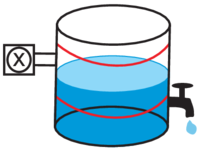
\includegraphics[width=0.6\textwidth]{images/watertank}
	\caption{Picture of possible Watertank configuration: Watertank that can get drained at all times and has a valve controlled by a control program~\cite{keymaeraGuide}.}
	\label{fig:watertank}
\end{figure}

The ``control'' part of this hybrid system is the valve, it can either drain the watertank with a rate of \(-2\) or it can fill the tank further with a rate of \(1\). The goal of the entire system then is, to keep the water level \(y\) of the tank between \(1\) and \(12\). Normally this is proven by \keym~ without actually implementing a control program. As our goal is to find a concrete implementation,  we first took a look at the hybrid model of the watertank. It is provided both in the form of a hybrid automata (See fig.~\ref{fig:watertank_ha}) and a hybrid program (See fig.~\ref{fig:watertank_hp}).

\begin{figure}
	\centering
	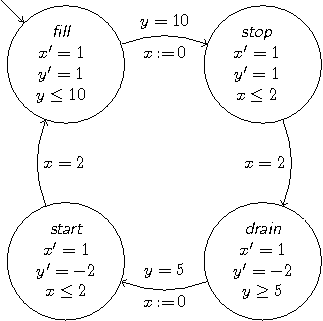
\includegraphics[width=0.6\textwidth]{images/watertank_ha}
	\caption{The Watertank CPS expressed as a hybrid automata~\cite{keymaeraGuide}.}
	\label{fig:watertank_ha}
\end{figure}

\begin{figure}
	\centering
	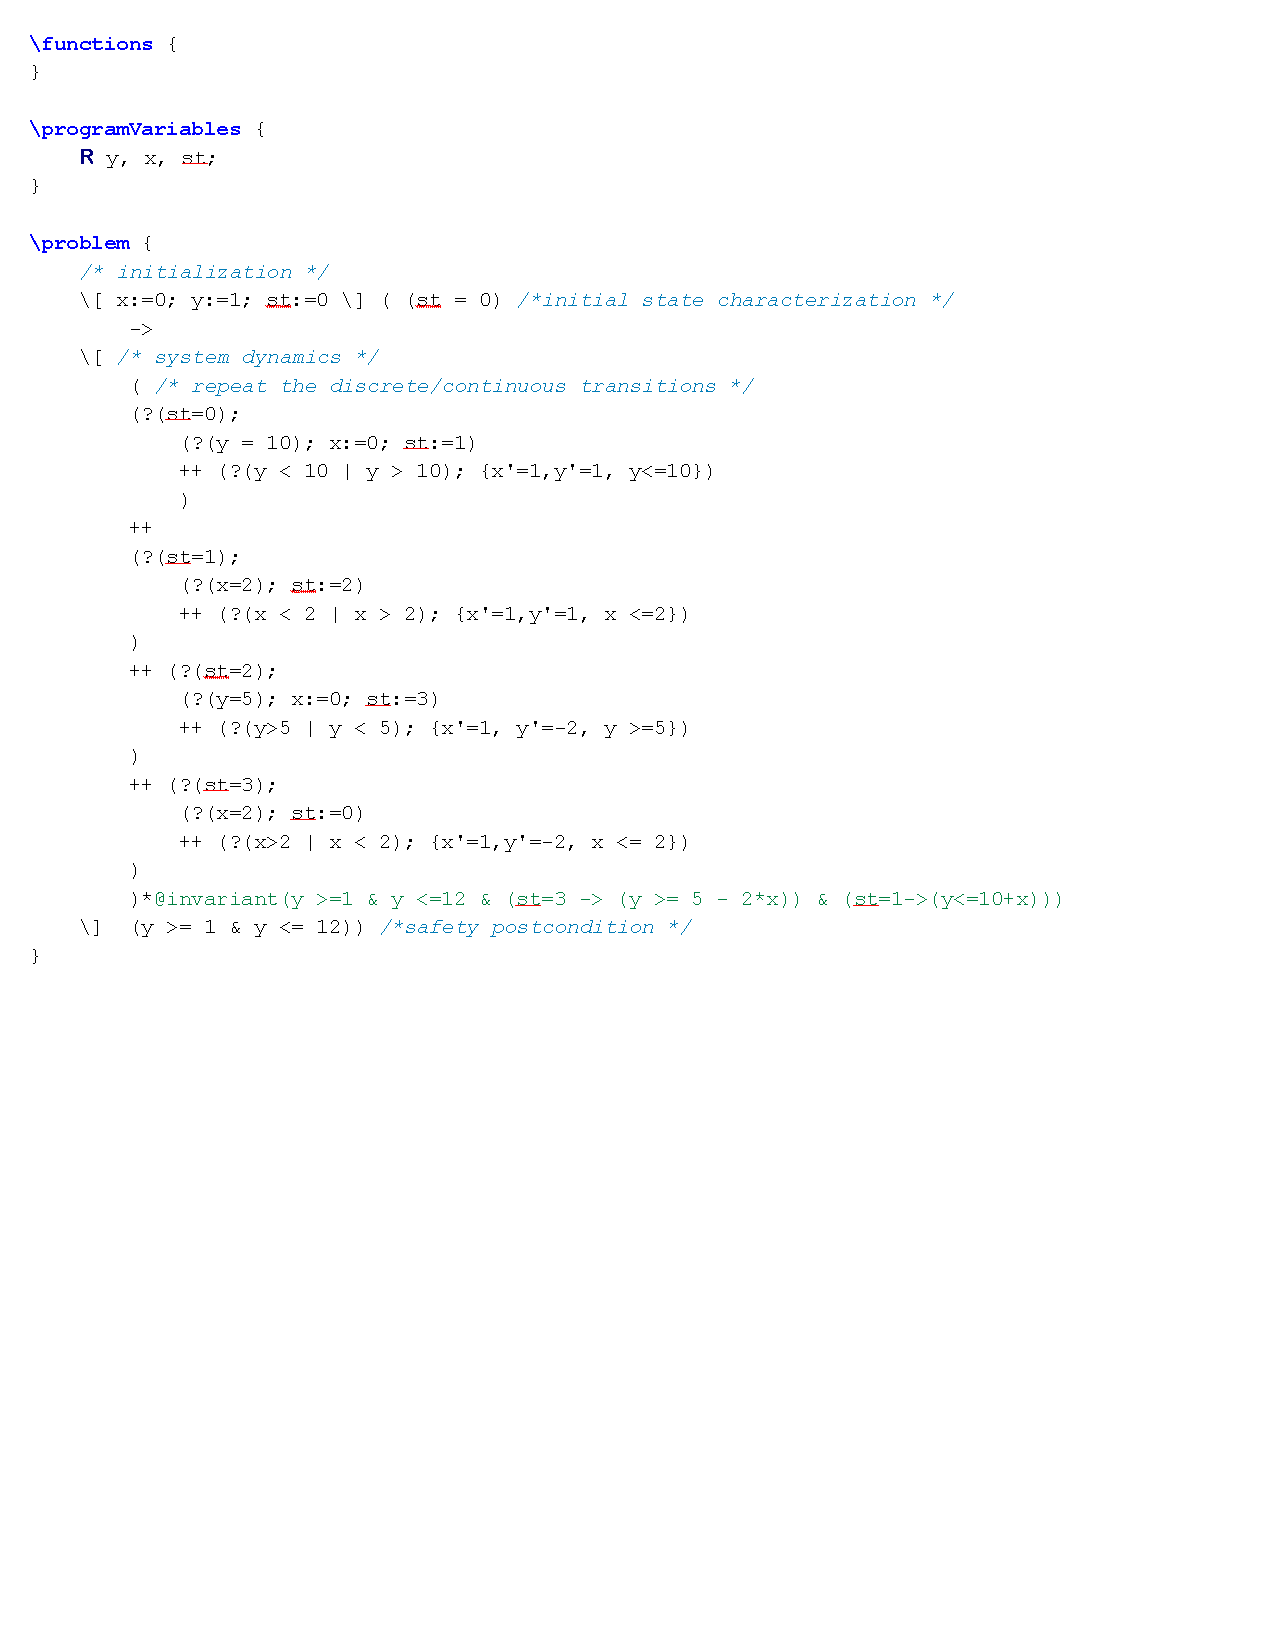
\includegraphics[width=0.8\textwidth]{images/watertank_hp}
	\caption{The Watertank CPS expressed as a hybrid program~\cite{keymaeraGuide}.}
	\label{fig:watertank_hp}
\end{figure}

\section{Finding the concrete Control Value Assisgnment}
\label{sec:Watertank:ControlValue}

In order to be able to apply Eq.~\ref{eq:Main_LogicRefinement} to this concrete example, the first challenge we faced was finding a spot in which a (or multiple) concrete control value is actually assigned. We call this assignment(s) the \textit{hook} as the actual implementation will ``hook'' into our hybrid model at this exact point. Taking a look at the Hybrid Automata describing the Watertank (See fig.~\ref{fig:watertank_ha}), it became obvious, that the hybrid model of the watertank required changing to be able to find our actual ``hook''. In the original model, a control value is never explicitly assigned, rather does the valve change its state non-deterministically, making a deterministical control program implementation impossible. Therefore, we tried to remodel the model to better serve our purpose, featuring a clear ticked hook that is called upon at deterministic times. (See fig.~\ref{fig:watertank_hp_ref}).

\begin{figure}
	\centering
	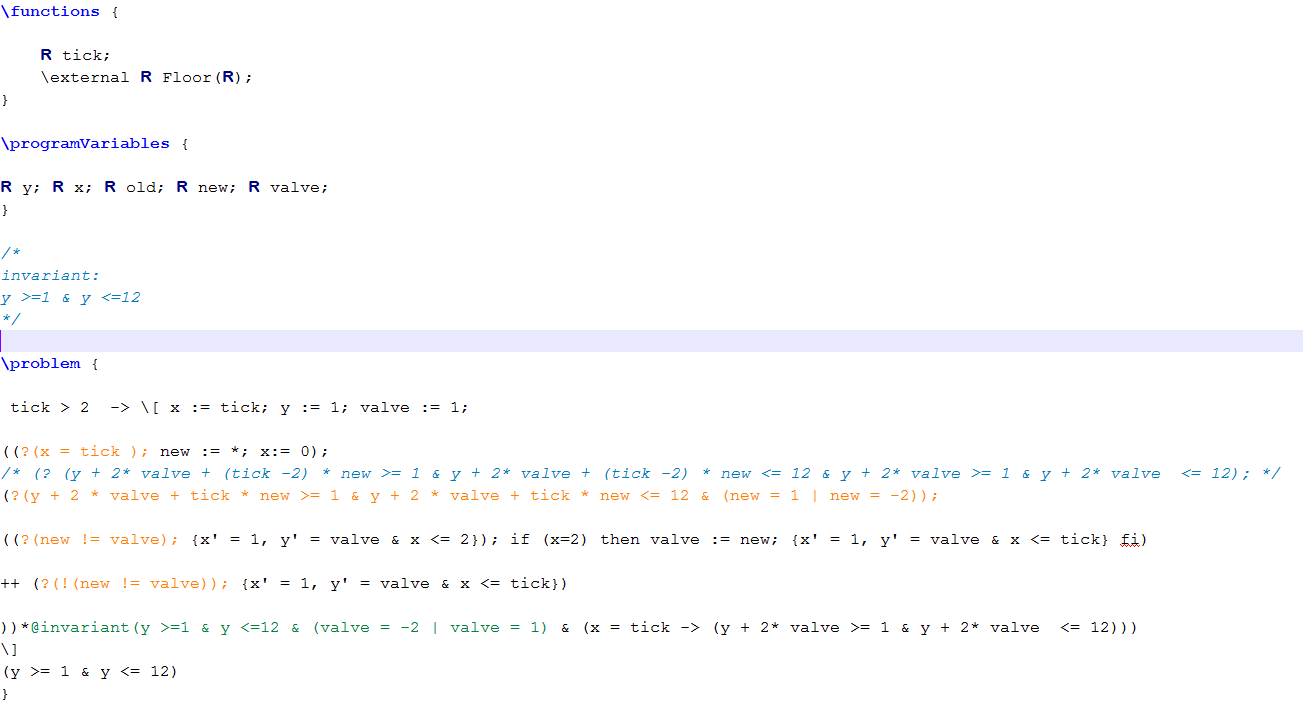
\includegraphics[width=0.9\textwidth]{images/watertank_hp_ref}
	\caption{The Watertank CPS after remodelling to account for hook.}
	\label{fig:watertank_hp_ref}
\end{figure}

We tried to keep the model mostly equivalent to the original, preserving the 2 clock ticks of time needed for the valve to change its state from drain to fill and vice-versa. This then proved difficult, when trying to think of possible implementations, as the program hook could be called again before the valve would have actually changed its state. To simplify this problem, we decided to only model cases in which the actual program tick (so the time between two hook calls)  is greater than 2 clock ticks (however long they may be).  This means, that the valve or control program doesn't have to have a (possibly infinite) list of the last control values assigned, which could be the case if the program was called more frequently than the valve is able to change states.

\section{Refining the original Hybrid Automata}
\label{sec:Watertank:Refinining}

\section{Finding the correct Program Safety Condition}
\label{sec:Watertank:SafetyCond}

The next step we attempted was finding the correct postcondition for the program hook (\(\psi\) in eq.~\ref{eq:Main_LogicRefinement}), which would then serve as the abstraction of the java control program we would later implement. This means, that the program would be built accordingly, so that it could be verified against this postcondition. The original postcondition we devised:

\begin{equation}
	\centering
	\begin{split}
		\psi \equiv ?( y + 2* valve + tick -2 * new  >= 1~\&~ \\ 2 * valve * (tick - 2) * new <= 12~\&~ \\  y + 2* valve >= 1~\&~ y + 2 * valve <= 12) 
	\end{split}
\label{eq:postCondOrig}
\end{equation}

When trying to verify the entire hybrid program (see comment in line 5 of the problem in fig.~\ref{fig:watertank_hp_ref}), this postcondition did not work. This means, that even in such a simple CPS as this watertank control system, finding the hook postcondition was non-trivial and only with the help of \keym's counterexamples did we manage to find the correct postcondition (See eq.~\ref{eq:postCondOrigCorrect}). 

\begin{equation}
	\centering
	\begin{split}
		\psi \equiv (?(y + 2 * valve + tick * new >= 1~\& \\ y + 2 * valve + tick * new <= 12~\& \\(new = 1 | new = -2))
	\end{split}
	\label{eq:postCondOrigCorrect}
\end{equation}

\keym~ verified our new hybrid program fully automatically (See fig.~\ref{fig:KeymaeraVerWatertank}).

\begin{figure}
	\centering
	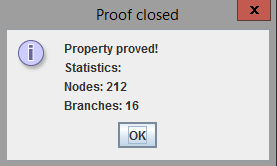
\includegraphics[width=0.6\textwidth]{images/watertank_keym_ver}
	\caption{The result of automatic verification by \keym~ of the Watertank hybrid program that includes our hook (See fig~\ref{fig:watertank_hp_ref}).}
	\label{fig:KeymaeraVerWatertank}
\end{figure}

\section{The (simple) Java Control Program}
\label{sec:Watertank:Java}

After completing verification of our hybrid model with \keym, we proceeded to implement a (simple) control program for the Watertank. Finding a suitable implementation proved difficult, as a parallel implementation (Both the control system and the differential equations working in parallel, modifying the water level) seemed more intuitive. This would defeat the purpose of actually finding a suitable hook and was more based on our understanding of the original hybrid model and not our version including the hook.

Using our understanding of a singular hook of the control system into the Watertank as well as the hook postcondition from the previous section as our specification for the actual control method, that would return the control value to the Watertank's valve, we then managed to implement a suitable discrete control method (See fig.~\ref{fig:source_controlMethod}).

\lstset{language=Java}
\begin{lstlisting}
public int getControlValue (int y, int old) {
		//Waterlevel in two time units
		int inTwo = y + 2 * old;
		//If we are raising level, keep raising if possible without hitting max_level before next tick
		if (old == 10) {
			if (inTwo + tick * 1 <= 116) {
				return 10;
			}
			else {
					return -20;
			}
		}
		//ELSE if we are currently lowering level, keep lowering if we can lower further without hitting min_level b4 next tick
		else {
			if (old == -20) {
				if (inTwo - tick * 2 >= 12) {
					return -20;
				}
				else {
						return 10;
				
				}
		
			}
		}
		//Only returned if old != 10 && old != -20, unreachable.
		return 0;
}
}
	%\label{lst:source_control_method}
\end{lstlisting}

\begin{figure}
	\centering
	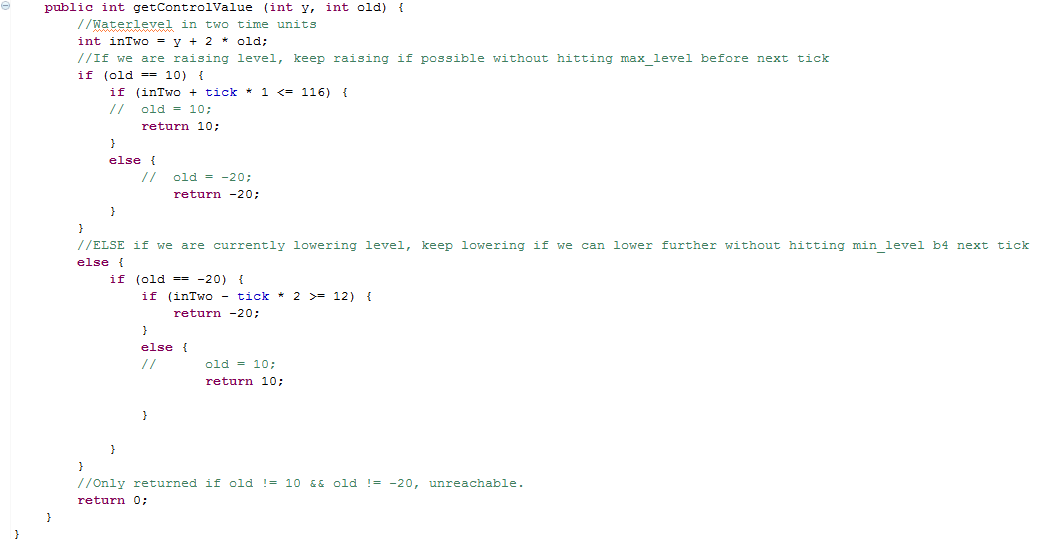
\includegraphics[width=0.9\textwidth]{images/source_control_method}
	\caption{The actual control method implemented.}
	\label{fig:source_controlMethod}
\end{figure}
The control method consists only of simple if-else-statements and just assigns the best-case (keep raising level if we were raising, keep lowering if we are lowering as long as postcondition is still valid) value to the valve.
For testing purposes, we also implemented a complete simulator of the Watertank CPS (See app.~\ref{app:fig:source_sim}).

\section{Finding the glue between Java and the Hybrid Model of the system}
\label{sec:Watertank:Glue}

The most important and also difficult part of our process, was finding the glue between the real parts of the hybrid system and our java control program. As real values (used in the hybrid model) and discrete values (used in our java implementation) are fundamentally different, a certain transformation has to occur.  In the Watertank example, this means, that the waterlevel as well as the last valve-value (be it fill or drain), which are passed to the control method, have to be converted into one direction by the glue. 

Also, the result of the computation in the method (so the new valve value) has to be converted in the other direction. In general the glue is not necessarily a bijective function, as some values will not exist in both worlds, making it a relation. For the Watertank, fortunately, this problem doe not exist, so finding a function translating the waterlevel and valve values into each other proved relatively easy. 

As we went along, we figured out how a general glue proof should look (See fig.~\ref{eq:glueGeneral}). Here \(x\) are the discrete values in our control program, \(y\) are the real world values, \(\psi\) is the postcondition of the control program expressed using discrete values and \(\phi\) is the actual safety condition we want to show for the entire hybrid system.

\begin{equation}
	\centering
	\begin{split}
		\forall x \in (Discrete World)~\forall y \in (Real World):(x,y) \in \textit{glue} \implies \psi(x) \implies \phi(y)
	\end{split}
	\label{eq:glueGeneral}
\end{equation}

Following this basic guideline, we were able to find a suitable glue relation (or in our case a bijective function) for this cps (See eq.~\ref{eq:glueWatertank}).

\begin{equation}
	\centering
	\begin{split}
		\forall y \in \mathbb{R} . \forall y_j \in \mathbb{Z}. \forall valve \in \mathbb{R}. \forall tick \in \mathbb{R}. \forall tick_j \in \mathbb{Z} . \forall new \in \mathbb{Z}. \forall result \in \mathbb{R} : \\  ((y_j = \textrm{floor}(10 * y) \wedge old_j = \textrm{floor}(10*valve) \wedge tick_j = \textrm{floor}(10*tick) \wedge result = 10 * new \wedge \\ y >= 1 \wedge y <= 12 \wedge (valve = 1  \vee valve = -2) \wedge tick > 2 \implies \\  ((result * tick_j/10 + y_j + 2 * old_j <= 116 \wedge result * tick_j/10 + y_j + 2 * old_j >= 12 \wedge \\ (result = 10 \vee result = -20)) \implies \\ y + 2 * valve + tick * new >= 1 \wedge y + 2 * valve + tick * new <= 12 \wedge \\ (new = 1 \vee new = -2))
	\end{split}
	\label{eq:glueWatertank}
\end{equation}

Thinking back to our implementation explained int he previous section, we can see
\section{Verification based on \keym}
\label{sec:Watertank:Verification}



%%%%%%%%%%%%%%%%%%%%%%%%%%%%%%%%%%%%%%%%%%%%%%%%%%%%%%%%%%%%%%%%%%%%%
%--PROCESS--%
%%%%%%%%%%%%%%%%%%%%%%%%%%%%%%%%%%%%%%%%%%%%%%%%%%%%%%%%%%%%%%%%%%%%%
\chapter{Introduction of formalized process of using Refinement to gain a concrete implementation from a hybrid model}
\label{ch:Process}

What the Watertank example shows is the non-triviality of refining the hybrid model into an implementation and of the verification of all necessary parts. Overall it is obvious, that a formalized approach to the general problem presented in chapter~\ref{ch:Introduction} is necessary. In this chapter we present a possible formalized approach to the problem, that we deem feasible.
\\

To aid readability we will now give an overview of the process without explanation, then detailing each step in the following sections. 

\begin{enumerate}
\item Abstraction of the original hybrid model to better split actual control system ``hook'' and physical evolutions.
\item Finding the necessary safety condition of the control value for verification with \keym.
\item Implementing control program according to safety condition as its specification and Verification by \key.
\item Finding the correct ``glue'' between hybrid model and control program and its verification by \keym.
\item Result validation: Was eq. ~\ref{eq':Main_LogicRefinement} proven?
\end{enumerate}

\section{Abstracting original hybrid model to better split actual control system ``hook'' and physical evolutions}
\label{sec:Process:Hook}
Most CPS we took a look at (See \cite{keymaera} Tutorial, \cite[p.~5, p.~11]{platzer2010b} \dots) as examples, did not have a concrete spot in which a control program could ``hook'' in easily. This means, that the first step in our refinement process has to be finding a suitable hook for the control program, referring to one or more non-deterministic assignments of a/multiple control values.

\section{Finding the necessary safety condition of the control value for verification with \keym}
\label{sec:Process:SafetyCond}

\section{Implementing control program according to safety condition as its specification and Verification by \key.}
\label{sec:Process:Implementation}

\section{Finding the correct glue between hybrid model and control program and verifying it with \keym}
\label{sec:Process:Glue}

\section{Evaluating results}
\label{sec:Process:Eval}










%% -------------------
%% | Example content |
%% -------------------
\iffalse
The content chapters of your thesis should of course be renamed. How many
chapters you need to write depends on your thesis and cannot be said in general.

Check out the examples theses in the SDQWiki:

\url{https://sdqweb.ipd.kit.edu/wiki/Abschlussarbeit/Studienarbeit}

Of course, you can split this .tex file into several files if you prefer. 


\section{First Section}
\label{sec:FirstContent:FirstSection}

\dots

\section{Second Section}
\label{sec:FirstContent:SecondSection}

\dots


\chapter{Second Content Chapter}
\label{ch:SecondContent}

\dots

\section{First Section}
\label{sec:SecondContent:FirstSection}

\dots

\section{Second Section}
\label{sec:SecondContent:SecondSection}

\dots

Add additional content chapters if required by adding new .tex files in the
\code{sections/} directory and adding an appropriate 
\code{\textbackslash include} statement in \code{thesis.tex}. 
\fi
%% ---------------------
%% | / Example content |
%% ---------------------